\documentclass[CJKmath,a4paper,10pt]{exam-zh}
\usepackage{geometry}
%\geometry{inner=1.5cm,outer=1.5cm,top=2.45cm,bottom=1cm}
\usepackage[dvipsnames,svgnames,x11names,table]{xcolor}

%\usepackage{amsmath,amssymb}
%\RequirePackage{unicode-math} % Math fonts in xetexorluatex
%\setmathfont{texgyrepagella-math.otf}
%\setmainfont{STIXTwoText}[
%	Path=./fonts/STIXTwoText/,
%  Extension = .otf,
%  UprightFont = STIXTwoMath-Regular,
%  BoldFont = STIXTwoText-SemiBold,
%  ItalicFont = STIXTwoText-Italic,
%  BoldItalicFont = STIXTwoText-BoldItalic,
%]
%\setmathfont{STIXTwoMath-Regular.otf}

\usepackage{tikz,calc}
\usetikzlibrary{calc,arrows,shadows.blur,tikzmark,angles,quotes,arrows.meta} % 角度、箭头库
% By default all math in TikZ nodes are set in inline mode. Change this to
% displaystyle so that we don't get small fractions.
\everymath{\displaystyle}

\usepackage[most]{tcolorbox}
\tcbuselibrary{breakable, skins,theorems}


\usepackage{xkeyval}
\makeatletter 
%\usepackage{amsmath,amssymb,amsthm}
\usepackage{xkeyval} 
\tcbset{
    common/.style={
      fontupper=\rmfamily,
      lower separated=true,
      coltitle=black,
      colback=gray!5,
      boxrule=0.1pt,
      fonttitle=\bfseries,
      enhanced,
      breakable,
      top=8pt,
      before skip=8pt,
      attach boxed title to top left={yshift=-0.05in,xshift=0.15in},
      boxed title style={
      	boxrule=0pt,
        colframe=black,
        arc=0pt,
        outer arc=0pt,
        drop fuzzy shadow
     	},
      separator sign={.},
      drop fuzzy shadow
     },
    litistyle/.style={
     	%例题风格
     	common,
     	colframe=gray,% 
     	colback=white,
     	colbacktitle=Gold,
     	sharp corners,rounded corners=southeast,
     	overlay unbroken and last={
     		\node[anchor=south east, outer sep=0pt] at (\linewidth-width,0){\textcolor{black!60}{$\blacksquare$}};
     	}
    },
% -----------------------------------------------------------------------------
% Explanation: BreakableBox@title key
% The following defines a pgfkeys/tcolorbox key named
%   "BreakableBox@title" which accepts 2 arguments (see 
%   "/.code n args={2}"). When the key is used like
%   "BreakableBox@title={<env>}{<optTitle>}" the code below is executed
%   with #1=<env> and #2=<optTitle>.
%
% Purpose:
% - If the second argument (#2) is empty, set the tcolorbox title to
%     \csname <env>name\endcsname~\thetcbcounter
%   which expands to the environment name (e.g. "liti" -> \litiname)
%   followed by the current counter value.
% - If the second argument is provided, append " (#2)" to the title.
%
% Notes:
% - This relies on \makeatletter being active so that keys with '@'
%   are allowed in control sequence names.
% - \ifblank is used to test whether #2 is empty; ensure the package
%   that provides \ifblank (for example, etoolbox or xparse) is loaded
%   earlier if necessary.
% - Example usage inside the code: \tcbset{title={...}} sets the
%   tcolorbox title key accordingly.
%
         BreakableBox@title/.code n args={2}
              {
                \ifblank{#2}
                  {\tcbset{title={\csname #1name\endcsname~\thetcbcounter}}}
                  {\tcbset{title={\csname #1name\endcsname~\thetcbcounter\ (#2)}}}
              },
}      
  % define an internal control sequence \newbreakablebox for fancy mode's newtheorem
  % #1 is the environment name, #2 is the prefix of label, #3 is the style
  % style: thmstyle, defstyle, prostyle
  % e.g. \newbreakablebox{theorem}{thm}{thmstyle}
  % will define two environments: numbered ``theorem'' and no-numbered ``theorem*''
  % WARNING FOR MULTILINGUAL: this cs will automatically find \theoremname's definition,
  % WARNING FOR MULTILINGUAL: it should be defined in language settings.
  \newcommand{\newbreakablebox}[3]{
    \ifcsundef{#1name}{%
      % define a default name if not defined before
      \tcbset{BreakableBox@title/.code n args={2}{\tcbset{title={use newcommand define #1name}}} }
    }{\relax}
    \DeclareTColorBox[auto counter]{#1}{ g o t\label g }{
        common, % use common style
        #3, % use the style passed in
        IfValueTF={##1}
          {BreakableBox@title={#1}{##1}}
          {
            IfValueTF={##2}
            {BreakableBox@title={#1}{##2}}
            {BreakableBox@title={#1}{}}
          },
        IfValueT={##4}
          {
            IfBooleanTF={##3}
              {label={##4}}
              {VIVID@label={#2}{##4}}
          }
      }
    \DeclareTColorBox{#1*}{ g o }{
        common,#3,
        IfValueTF={##1}
          {BreakableBox@title={#1}{##1}}
          {
            IfValueTF={##2}
            {BreakableBox@title={#1}{##2}}
            {BreakableBox@title={#1}{}}
          },
      }
  }
% define several environment 
% we define headers like \definitionname before
\newcommand{\litiname}{例题}
\newbreakablebox{liti}{def}{litistyle}
  
  
%补充内容
%%设置新字体
%%定义带圈数字命令
\newfontfamily{\nmfont}{circlenumber}
[%
Extension=.otf,
Path=./fonts/]

\newcommand{\quan}[1]{{\nmfont \symbol{#1}}}
\newcommand{\kk}[1]{\quan{\numexpr32+#1}}%\kk{<参数范围1-95>}96、97、98、99分别用\quan{196} \quan{197} \quan{199} \quan{201}

%脚注使用带圈数字
\newcommand*\kkctr[1]{%
  \protect\kk{\number\numexpr\value{#1}\relax}}
\renewcommand*\thefootnote{\textcolor{black}{\kkctr{footnote}}}

%%无悬挂脚注格式
\renewcommand\@makefntext[1]{%
  \setlength\parindent{2\ccwd}\selectfont
  \@thefnmark\ #1}

%修改\part，使其不分页
\def\@endpart{%
	\thispagestyle{empty}
  \vskip40\p@%
   \@afterheading}



\RequirePackage{enumitem}
%\newenvironment{myenum}{\begin{enumerate}[label=\protect\kk{\arabic*}]\small}{\end{enumerate}}%
\setlist{noitemsep}
\setlist[enumerate, 1]{label=\protect\kk{\arabic*},itemsep=0.5ex}  
\makeatother



%%%marker环境
\newtcolorbox{marker}[1][]{enhanced,before skip=2mm,
	after skip=3mm,fontupper=\rmfamily,
	boxrule=0.4pt,left=5mm,right=2mm,top=1mm,bottom=1mm,
	colback=yellow!50,colframe=yellow!20!black,
	sharp corners,rounded corners=southeast,
	arc is angular,arc=3mm,underlay={%
		\path[fill=tcbcolback!80!black] ([yshift=3mm]interior.south east)--++(-0.4,-0.1)--++(0.1,-0.2);
		\path[draw=tcbcolframe,shorten <=-0.05mm,shorten >=-0.05mm] ([yshift=3mm]interior.south east)--++(-0.4,-0.1)--++(0.1,-0.2);
		\path[fill=yellow!50!black,draw=none] (interior.south west) rectangle node[white]{\Huge\bfseries !} ([xshift=4mm]interior.north west);
	},
	drop fuzzy shadow,#1
}


\usepackage{graphicx}
\usepackage{float}

% 使用 exam-zh 官方参数设置页脚文字
\examsetup{page={foot-content={物理习题第;页（共~;页）}}}

\begin{document}



\section{物理}
% 绘制斜面+物块示意图
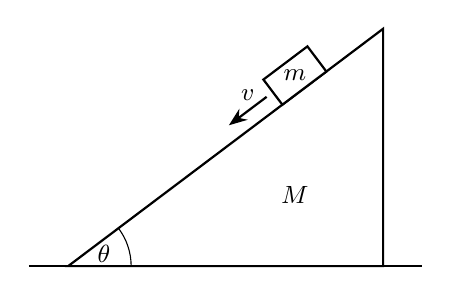
\begin{tikzpicture}[>=Stealth,        % 箭头样式
	%scale=1.2,        % 缩放比例
	every node/.style={font=\small} % 节点字体大小
	]
	
	% 定义基本参数
	\def\ang{37} % 倾角
	\def\w{4}    % 底边长
	\pgfmathsetmacro{\h}{\w*tan(\ang)} % 高
	
	% 坐标定义
	\coordinate (A) at (0,0);
	\coordinate (B) at (\w,0);
	\coordinate (C) at (\w,\h);
	
	% 绘制斜面体
	\draw[thick] (A) -- (B) -- (C) -- cycle;
	% 标注M
	\node at ($(A)!0.6!(B)!0.3!(C)$) {$M$};
	
	% 标注角度
	\draw pic["$\theta$", draw, angle radius=0.8cm] {angle=B--A--C};
	
	% 绘制物块 (放置在斜面上半部分)
	\coordinate (P) at ($(A)!0.75!(C)$); % 位置在斜面75%处
	\begin{scope}[shift={(P)},rotate=\ang]
		\draw[thick,fill=white] (-0.35,0) rectangle (0.35,0.4);
		\node at (0,0.2) {$m$};
		% 速度箭头 v
		\draw[->,thick] (-0.45,0.2) -- ++(-0.6,0) node[midway,above] {$v$};
	\end{scope}
	
	% 绘制地面
	\draw[thick] (-0.5,0) -- (\w+0.5,0);
	
\end{tikzpicture}
\begin{liti}
如图所示，质量为$M$、倾角为$\theta$的斜面静止在水平地面上，质量为$m$的物块沿斜面以加速度$a$匀加速下滑，现给$m$加一竖直向下的恒力$F$，$M$仍静止，则下列说法正确的是（）

\begin{enumerate}
	\item[A.] 未加$F$之前，$M$对地面的压力大小为$(M+m)g$
	\item[B.] 未加$F$之前，$M$对$m$作用力大小为$m\sqrt{a^2+g^2}$
	\item[C.] 加力$F$之后，$m$加速度大于$a$
	\item[D.] 加力$F$之后，地面对$M$的摩擦力增大了$F\dfrac{a}{g}\cos\theta$
\end{enumerate}
\tcblower
\textbf{解：}

\begin{itemize}
	\item \textbf{A选项：} 对$M$、$m$整体分析，整体在竖直方向上有向下的加速度分量$a_y = a\sin\theta$，处于失重状态，故地面对$M$的支持力$N < (M+m)g$，由牛顿第三定律，压力小于$(M+m)g$，A错误。
	\item \textbf{B选项：} 未加$F$之前，$M$对$m$的作用力$\vec{F}_{Mm}$与重力$m\vec{g}$的合力提供$m$的合外力$m\vec{a}$，即$\vec{F}_{Mm} + m\vec{g} = m\vec{a}$。由矢量运算法则，$|\vec{F}_{Mm}| = \sqrt{(mg)^2 + (ma)^2 - 2mg\cdot ma \cos(90^\circ-\theta)} = m\sqrt{g^2+a^2-2ga\sin\theta}$，B错误。
	\item \textbf{C选项：} 加力$F$相当于将重力加速度增大为$g' = g + \frac{F}{m}$。原加速度$a = g(\sin\theta - \mu\cos\theta)$，新加速度$a' = (g+\frac{F}{m})(\sin\theta - \mu\cos\theta) = a + \frac{F}{m}\cdot \frac{a}{g} > a$，C正确。
	\item \textbf{D选项：} 对$M$、$m$整体，水平方向只受地面对$M$的摩擦力$f$，由牛顿第二定律，$f = m a_x = m a \cos\theta$。加力$F$后，新的摩擦力$f' = m a' \cos\theta = m (a + \frac{Fa}{mg}) \cos\theta = f + \frac{Fa}{g}\cos\theta$。增加量$\Delta f = \frac{Fa}{g}\cos\theta$，D正确。
\end{itemize}

故选：\textbf{CD}。

\begin{enumerate}
	\item \textbf{A选项深入分析（失重现象）：}

我们通过\textbf{整体法}来定量推导地面对$M$的实际支持力。

\begin{enumerate}
    \item \textbf{受力分析：} 把斜面$M$和物块$m$看作一个整体。系统在竖直方向收到向下的总重力 $(M+m)g$ 和向上的支持力 $N$。
    \item \textbf{加速度分析：}
    \begin{itemize}
        \item 斜面$M$静止，竖直加速度为 $0$。
        \item 物块$m$沿斜面加速下滑，加速度大小为 $a$。其竖直向下的分量为 $a_y = a\sin\theta$。
    \end{itemize}
    \item \textbf{列牛顿第二定律方程（竖直方向，向下为正）：}
    \[ (M+m)g - N = M \cdot 0 + m \cdot (a\sin\theta) \]
    \item \textbf{求解支持力：}
    \[ N = (M+m)g - m a \sin\theta \]
\end{enumerate}

\textbf{结论：}由于 $m, a, \sin\theta$ 均为正值，故支持力 $N < (M+m)g$。说明系统处于\textit{失重}状态（整体质心有向下的加速度），A选项错误。

\item 
\textbf{B选项深入分析（力的矢量三角形）：}

题目询问的是$M$对$m$的作用力，即支持力$N'$与摩擦力$f$的合力，记为$\vec{F}_{Mm}$。

\begin{enumerate}
    \item \textbf{牛顿第二定律分析：} 物块$m$受到重力$m\vec{g}$和$M$的作用力$\vec{F}_{Mm}$，两者的合力提供沿斜面向下的加速度$m\vec{a}$。
    \[ \vec{F}_{Mm} + m\vec{g} = m\vec{a} \quad \Rightarrow \quad \vec{F}_{Mm} = m\vec{a} - m\vec{g} \]
    \item \textbf{矢量运算法则（余弦定理）：}
    我们要求的是矢量差的模长。
    \begin{itemize}
        \item 矢量$m\vec{a}$的大小为$ma$，方向沿斜面向下。
        \item 矢量$m\vec{g}$的大小为$mg$，方向竖直向下。
        \item 两个矢量之间的夹角为$90^\circ - \theta$（因为斜面与水平面夹角为$\theta$）。
    \end{itemize}
    根据余弦定理（矢量减法）：
    \[ |\vec{F}_{Mm}|^2 = (ma)^2 + (mg)^2 - 2(ma)(mg)\cos(90^\circ - \theta) \]
    \[ |\vec{F}_{Mm}| = m\sqrt{a^2 + g^2 - 2ag\sin\theta} \]
\end{enumerate}

\textbf{结论：} 只有当$\theta=0^\circ$（水平面上加速）时，结果才可能是$m\sqrt{a^2+g^2}$。题目给出的表达式忽略了能够体现方向的交叉项$-2ag\sin\theta$，故B选项错误。

\item 
\textbf{C选项深入分析（等效重力法）：}

\begin{enumerate}
    \item \textbf{原状态：} 物块只受重力 $mg$ 和斜面作用力。加速度为：
    \[ a = \frac{mg\sin\theta - \mu mg\cos\theta}{m} = g(\sin\theta - \mu\cos\theta) \]
    \item \textbf{加力后：} 物块受到竖直向下的恒力 $F$。可以将 $F$ 视为物块增加的“重力”。
    此时等效重力加速度为 $g' = g + \dfrac{F}{m}$。
    \item \textbf{新加速度：} 将 $g$ 替换为 $g'$：
    \[ a' = g'(\sin\theta - \mu\cos\theta) = \left(g + \dfrac{F}{m}\right)(\sin\theta - \mu\cos\theta) \]
    \[ a' = a + \dfrac{F}{m}(\sin\theta - \mu\cos\theta) \]
    由于物体能加速下滑，说明 $(\sin\theta - \mu\cos\theta) > 0$，\textbf{且$F, m > 0$}，所以 $a' > a$，C选项正确。
\end{enumerate}

\item 
\textbf{D选项深入分析（整体法求摩擦力）：}

\begin{enumerate}
    \item \textbf{受力分析：} 选取斜面$M$和物块$m$组成的整体为研究对象。考虑水平方向的受力与运动。
    \item \textbf{加力前：}
    \begin{itemize}
        \item 水平方向受力：地面对$M$的静摩擦力 $f$。
        \item 水平方向牛顿第二定律：
        \[ f = M \cdot a_{M,x} + m \cdot a_{m,x} \]
        因$M$静止，$a_{M,x}=0$；$m$的水平加速度 $a_{m,x} = a\cos\theta$。
        \[ f = m a \cos\theta \]
    \end{itemize}
    \item \textbf{加力后：}
    \begin{itemize}
        \item 物块加速度变为 $a'$。根据C选项分析， $a' = a\left(1 + \dfrac{F}{mg}\right)$。
        \item 新的摩擦力 $f'$：
        \[ f' = m a' \cos\theta = m \left[ a \left( 1 + \dfrac{F}{mg} \right) \right] \cos\theta \]
        \[ f' = m a \cos\theta + \dfrac{F a}{g} \cos\theta = f + \dfrac{F}{g} a \cos\theta \]
    \end{itemize}
    \item \textbf{结论：} 摩擦力增加了 $\Delta f = \dfrac{F a}{g} \cos\theta$，D选项正确。
\end{enumerate}

\end{enumerate}

\end{liti}
\vspace{0.5cm}
\begin{center}
\begin{tikzpicture}[>=Stealth, scale=1, every node/.style={font=\small}]
    % 图1：m受力分析
    \begin{scope}
        \def\ang{37}
        \coordinate (O) at (0,0);
        % \draw[dashed] (-1,0) -- (3,0); % Horizontal line
        \draw[thick] (0,0) -- (3, {3*tan(\ang)});
        \node at (2.5, 2.3) {斜面};
        
        % Object
        \coordinate (P) at (1.5, {1.5*tan(\ang)});
        \begin{scope}[shift={(P)}, rotate=\ang]
            \draw[thick, fill=white] (-0.35,0) rectangle (0.35,0.4);
            \node at (0,0.2) {$m$};
            \coordinate (Center) at (0, 0.2);
            
            % Forces
            \draw[->, red, thick] (Center) -- (0, 1.2) node[above] {$N_m$}; % Support
            \draw[->, red, thick] (Center) -- (1.0, 0.2) node[right] {$f_m$}; % Friction (up slope)
        \end{scope}
        % Gravity
        \begin{scope}[shift={(P)}]
             \draw[->, blue, thick] (-0.2,{0.2*cos(\ang)}) -- (-0.2, -1.2) node[right] {$mg$};
        \end{scope}
        \node[below] at (1.5, -0.5) {图1：物块$m$受力分析};
    \end{scope}

    % 图2：M受力分析
    \begin{scope}[shift={(6,0)}]
        \def\ang{37}
        \def\w{3.5}
        \pgfmathsetmacro{\h}{\w*tan(\ang)}
        
        \coordinate (A) at (0,0);
        \coordinate (B) at (\w,0);
        \coordinate (C) at (\w,\h);
        
        \draw[thick] (A) -- (B) -- (C) -- cycle;
        \node at ($(A)!0.6!(B)!0.3!(C)$) {$M$};
        
        % Forces from m on M
        \coordinate (Contact) at ($(A)!0.65!(C)$);
        \begin{scope}[shift={(Contact)}, rotate=\ang]
            % N'_m (Pressure)
            \draw[->, violet, thick] (0,0) -- (0, -0.8) node[right] {$N'_m$};
            % f'_m (Friction from m, down slope)
            \draw[->, violet, thick] (0,0) -- (-0.8, 0) node[above left] {$f'_m$};
        \end{scope}
        
        % Gravity M
        \coordinate (MCenter) at (2, 0.8);
        \draw[->, blue, thick] (MCenter) -- ++(0, -1.2) node[right] {$Mg$};
        
        % Ground Support
        \draw[->, red, thick] (2, 0) -- (2, 1.5) node[left] {$N_{\text{地}}$};
        
        % Ground Friction (M pushed right by N'm_x and f'm_x? No. Check x components.)
        % N'm is perp to slope (down-right). +x component.
        % f'm is down slope (down-left). -x component.
        % If N'm_x > f'm_x, M tends right.
        % N'm_x = mg cos theta sin theta.
        % f'm_x = f'm cos theta = m(g sin theta - a) cos theta.
        % If a=g sin theta (smooth), f'm=0. M pushed right by N'm. Friction left.
        % Generally friction f_ground is left.
        \draw[->, red, thick] (2, 0) -- (0.8, 0) node[below] {$f_{\text{地}}$};
        
        \draw[thick] (-0.5,0) -- (\w+0.5,0);
        \node[below] at (2, -0.5) {图2：斜面$M$受力分析};
    \end{scope}
\end{tikzpicture}
\end{center}

\vspace{0.5cm}
\textbf{【补充】A选项的第二种解法：隔离法分析（验证结论）}

如果不使用整体法，我们可以分别隔离物块$m$和斜面$M$进行受力分析，过程虽然繁琐但能验证结论的正确性。

\begin{itemize}
	\item \textbf{1. 分析物块$m$（求 $m$ 对 $M$ 的作用力）：}
	\begin{itemize}
		\item 垂直斜面方向平衡：支持力 $N_{m} = mg\cos\theta$。
		\item 沿斜面方向牛顿第二定律：$mg\sin\theta - f_{m} = ma \Rightarrow$ 摩擦力 $f_{m} = m(g\sin\theta - a)$。
	\end{itemize}
	由牛顿第三定律，$m$施加给$M$的压力 $N'_{m} = mg\cos\theta$（垂直斜面向下），摩擦力 $f'_{m} = m(g\sin\theta - a)$（沿斜面向下）。
	
	\item \textbf{2. 分析斜面$M$（求地面对 $M$ 的支持力）：}
	斜面$M$处于静止状态，竖直方向受力平衡。
	\begin{itemize}
		\item 受到向下的力：重力 $Mg$，以及$m$的作用力的竖直分量。
		\item $N'_{m}$ 的竖直分量：$N'_{m}\cos\theta = mg\cos^2\theta$。
		\item $f'_{m}$ 的竖直分量：$f'_{m}\sin\theta = m(g\sin\theta - a)\sin\theta = mg\sin^2\theta - ma\sin\theta$。
	\end{itemize}
	地面对$M$的支持力 $N_{ground}$ 平衡上述所有向下的力：
	\[ N_{ground} = Mg + (N'_{m}\cos\theta) + (f'_{m}\sin\theta) \]
	代入表达式：
	\[ N_{ground} = Mg + mg\cos^2\theta + (mg\sin^2\theta - ma\sin\theta) \]
	合并 $mg(\cos^2\theta + \sin^2\theta)$：
	\[ N_{ground} = Mg + mg(1) - ma\sin\theta = (M+m)g - ma\sin\theta \]
\end{itemize}

\textbf{结论：} 隔离法得到的结果与整体法完全一致，地面对$M$的支持力小于总重力$(M+m)g$。
\newpage
\begin{liti}
如图所示，平静的海面上，两艘拖船$A$、$B$通过不可伸长的缆绳拖着驳船$C$运动，某时刻两根缆绳的夹角为$\theta$，两拖船$A$、$B$的速度大小分别为$2\ \text{m/s}$、$2.4\ \text{m/s}$。已知两拖船的运动方向始终沿缆绳方向，$\sin\theta = 0.8$，则此时驳船$C$的速度大小为\paren[A]
\begin{choices}
	\item $2.5\ \text{m/s}$
	\item $3.0\ \text{m/s}$
	\item $3.6\ \text{m/s}$
	\item $3.9\ \text{m/s}$
\end{choices}


\begin{center}
\begin{tikzpicture}[scale=1.0,>=stealth]
  % Geometry based on theta for a clean schematic
  \pgfmathsetmacro{\thetadeg}{53.13}
  \coordinate (C) at (0,0);
  \coordinate (A) at ({-3*sin(\thetadeg/2)}, {3*cos(\thetadeg/2)});
  \coordinate (B) at ({3*sin(\thetadeg/2)}, {3*cos(\thetadeg/2)});

  % Ropes
  \draw[thick] (C) -- (A);
  \draw[thick] (C) -- (B);

  % Angle theta
  \pic [draw, "$\theta$", angle radius=0.7, angle eccentricity=1.2] {angle = A--C--B};

  % Boats and barge (rect + triangle)
  \pgfmathanglebetweenpoints{\pgfpointanchor{A}{center}}{\pgfpointanchor{C}{center}}
  \let\angleA\pgfmathresult
  \pgfmathanglebetweenpoints{\pgfpointanchor{B}{center}}{\pgfpointanchor{C}{center}}
  \let\angleB\pgfmathresult
  \def\boatL{0.5}
  \def\boatW{0.2}
  \begin{scope}[shift={(A)}, rotate=\angleA+180]
    \draw[fill=gray!20] (-0.3,-0.1) rectangle (0.1,0.1);
    \draw[fill=gray!20] (0.1,-0.1) -- (0.3,0) -- (0.1,0.1) -- cycle;
  \end{scope}
  \begin{scope}[shift={(B)}, rotate=\angleB+180]
    \draw[fill=gray!20] (-0.3,-0.1) rectangle (0.1,0.1);
    \draw[fill=gray!20] (0.1,-0.1) -- (0.3,0) -- (0.1,0.1) -- cycle;
  \end{scope}
  \begin{scope}[shift={(C)}, rotate=90]
    \draw[fill=gray!20] (-0.35,-0.12) rectangle (0.15,0.12);
    \draw[fill=gray!20] (0.15,-0.12) -- (0.35,0) -- (0.15,0.12) -- cycle;
  \end{scope}
  \node[left] at (A) {$A$};
  \node[right] at (B) {$B$};
  \node[below] at ($(C)+(0,-0.3cm)$) {$C$};

  % Velocity arrows along ropes
  \draw[->, blue, thick] (C) -- ($(C)!0.6!(A)$) node[midway, above left] {$2\,\text{m/s}$};
  \draw[->, blue, thick] (C) -- ($(C)!0.6!(B)$) node[midway, above right] {$2.4\,\text{m/s}$};

  % C velocity
  \draw[->, red, thick] (C) -- (0,1.6) node[right] {$v_C$};

  \node[below] at (0,-1) {图3：拖船与驳船速度关系示意};
\end{tikzpicture}
\end{center}
\tcblower
设缆绳方向的单位向量分别为 $\mathbf{u}_A$、$\mathbf{u}_B$，夹角为 $\theta$。绳长不变意味着驳船$C$的速度在每根缆绳方向上的分量等于对应拖船的速度：
\[
\mathbf{v}_C\cdot \mathbf{u}_A = 2,\qquad \mathbf{v}_C\cdot \mathbf{u}_B = 2.4.
\]
用 $\mathbf{v}_C = x\mathbf{u}_A + y\mathbf{u}_B$ 表示，则
\[
\begin{cases}
x + y\cos\theta = 2,\\
x\cos\theta + y = 2.4.
\end{cases}
\]
解得
\[
x = \dfrac{2 - 2.4\cos\theta}{\sin^2\theta},\qquad y = \dfrac{2.4 - 2\cos\theta}{\sin^2\theta}.
\]
代入 $\sin\theta=0.8,\ \cos\theta=0.6$：
\[
x = \dfrac{2-1.44}{0.64}=0.875,\qquad y = \dfrac{2.4-1.2}{0.64}=1.875.
\]
驳船速度大小
\[
v_C^2 = x^2 + y^2 + 2xy\cos\theta
= 0.875^2 + 1.875^2 + 2\times 0.875\times 1.875\times 0.6 = 6.25.
\]
\[
v_C = 2.5\ \text{m/s}.
\]
\textbf{答案：}A.

\vspace{0.3cm}
\textbf{为什么不能直接用“余弦定理（向量相加）”：直观图}

\begin{center}
\begin{tikzpicture}[scale=1.0,>=stealth]
  % -------- Left: correct (projection constraints) --------
  \begin{scope}[shift={(-4.3,0)}]
    \coordinate (O) at (0,0);
    \coordinate (uA) at (2.2,0.5);
    \coordinate (uB) at (0.8,2.1);
    \coordinate (v)  at (1.6,2.4);

    \draw[->,thick] (O) -- (uA) node[right] {$\mathbf{u}_A$};
    \draw[->,thick] (O) -- (uB) node[above] {$\mathbf{u}_B$};
    \draw[->,red,thick] (O) -- (v) node[above right] {$\mathbf{v}_C$};

    % projections to uA and uB
    \coordinate (pA) at ($(O)!0.66!(uA)$);
    \coordinate (pB) at ($(O)!0.76!(uB)$);
    \draw[dashed,blue] (v) -- (pA);
    \draw[dashed,blue] (v) -- (pB);
    \node[blue] at (1.65,1.55) {$\mathbf{v}_C\cdot\mathbf{u}_A=2$};
    \node[blue] at (0.55,1.35) {$\mathbf{v}_C\cdot\mathbf{u}_B=2.4$};

    \pic [draw, "$\theta$", angle radius=0.45, angle eccentricity=1.25] {angle = uA--O--uB};
    \node[below] at (1.1,-0.7) {左：正确（投影约束）};
  \end{scope}

  % -------- Right: wrong (treat 2 and 2.4 as vector addition) --------
  \begin{scope}[shift={(2.4,0)}]
    \coordinate (O2) at (0,0);
    \coordinate (a2) at (2.2,0.5);
    \coordinate (b2) at (0.8,2.1);
    \coordinate (tip) at ($(a2)+(b2)$);

    \draw[->,thick,blue] (O2) -- (a2) node[right] {$2$};
    \draw[->,thick,blue] (O2) -- (b2) node[above] {$2.4$};
    \draw[->,thick,gray] (a2) -- (tip);
    \draw[->,thick,gray] (b2) -- (tip);
    \draw[->,red,thick] (O2) -- (tip) node[above right] {$\mathbf{v}_A+\mathbf{v}_B$};

    \pic [draw, "$\theta$", angle radius=0.45, angle eccentricity=1.25] {angle = a2--O2--b2};
    \node[below] at (1.4,-0.7) {右：错误（把影长当矢量相加）};
  \end{scope}
\end{tikzpicture}
\end{center}

\begin{itemize}
  \item 本题给的 $2,\ 2.4$ 是同一个速度 $\mathbf{v}_C$ 在两条缆绳方向上的\textbf{投影长度}，不是两个独立速度矢量。
  \item 余弦定理对应的是“已知两边及夹角，求第三边”的\textbf{同一三角形边长关系}；这要求 $2$ 和 $2.4$ 是两条真实矢量边。
  \item 这里应先写投影方程 $\mathbf{v}_C\cdot\mathbf{u}_A=2,\ \mathbf{v}_C\cdot\mathbf{u}_B=2.4$，再解出 $v_C$，而不是直接做矢量合成。
\end{itemize}

\textbf{点积法标准解（详细步骤）}

设驳船速度向量为 $\mathbf{v}$，两条缆绳方向的单位向量分别为 $\mathbf{u}_A,\mathbf{u}_B$，且两者夹角为 $\theta$。

由“缆绳不可伸长”可得：驳船在每条缆绳方向上的速度分量，分别等于对应拖船速度，故
\[
\mathbf{v}\cdot\mathbf{u}_A=2,\qquad \mathbf{v}\cdot\mathbf{u}_B=2.4.
\]

把 $\mathbf{v}$ 在 $\mathbf{u}_A,\mathbf{u}_B$ 张成的平面内展开：
\[
\mathbf{v}=x\mathbf{u}_A+y\mathbf{u}_B.
\]
两边分别与 $\mathbf{u}_A,\mathbf{u}_B$ 点乘，并利用
\[
\mathbf{u}_A\cdot\mathbf{u}_A=1,\quad \mathbf{u}_B\cdot\mathbf{u}_B=1,\quad \mathbf{u}_A\cdot\mathbf{u}_B=\cos\theta,
\]
得方程组
\[
\begin{cases}
x+y\cos\theta=2,\\
x\cos\theta+y=2.4.
\end{cases}
\]
解得
\[
x=\dfrac{2-2.4\cos\theta}{\sin^2\theta},\qquad
y=\dfrac{2.4-2\cos\theta}{\sin^2\theta}.
\]
代入 $\sin\theta=0.8,\ \cos\theta=0.6$：
\[
x=\dfrac{2-1.44}{0.64}=0.875,\qquad
y=\dfrac{2.4-1.2}{0.64}=1.875.
\]

再由
\[
v^2=\mathbf{v}\cdot\mathbf{v}=(x\mathbf{u}_A+y\mathbf{u}_B)\cdot(x\mathbf{u}_A+y\mathbf{u}_B)
=x^2+y^2+2xy\cos\theta,
\]
得
\[
v^2=0.875^2+1.875^2+2\times0.875\times1.875\times0.6=6.25.
\]
\[
v=2.5\ \text{m/s}.
\]
故驳船速度大小为 $2.5\ \text{m/s}$（选A）。
\end{liti}

\begin{liti}
\begin{minipage}{.6\linewidth}
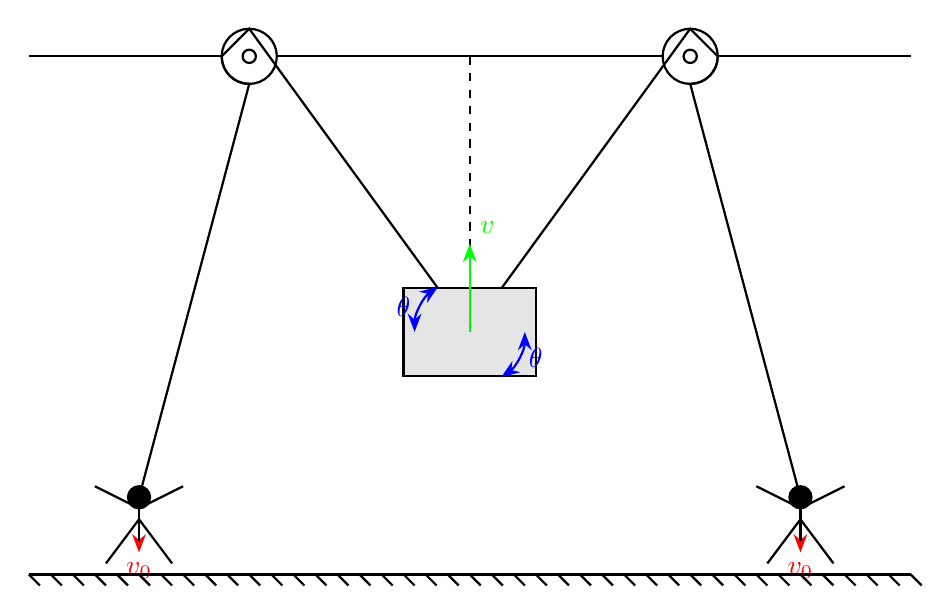
\begin{tikzpicture}[>=Stealth, thick, scale=1.4]
	% 顶部固定横梁
	\draw (-4, 1.5) -- (4, 1.5);
	
	% 两个定滑轮（带轮轴，绳子绕滑轮边缘）
	\draw[fill=white] (-2, 1.5) circle (0.25); % 左侧滑轮
	\draw (-2, 1.5) circle (0.06); % 滑轮轴
	\draw[fill=white] (2, 1.5) circle (0.25);  % 右侧滑轮
	\draw (2, 1.5) circle (0.06); % 滑轮轴
	
	% 木箱中心坐标
	\coordinate (box) at (0, -1);
	
	% 绳子路径（绕滑轮边缘，而非穿圆心）
	% 左侧绳子：地面人手 → 滑轮下边缘 → 木箱
	\draw (-3, -2.5) -- (-2, 1.25) arc(270:180:0.25) -- (-2, 1.75) -- (box);
	% 右侧绳子：地面人手 → 滑轮下边缘 → 木箱
	\draw (3, -2.5) -- (2, 1.25) arc(270:360:0.25) -- (2, 1.75) -- (box);
	
	% 木箱（矩形）
	\draw[fill=gray!20] (box) +(-0.6, -0.4) rectangle +(0.6, 0.4);
	
	% 角度标注（绳子与竖直方向的夹角θ）
	\draw[dashed] (0, 1.5) -- (box); % 竖直参考线
	\draw[<->, blue] (box) +(0.5, 0) arc(0:-55:0.5) node[midway, right] {$\theta$};
	\draw[<->, blue] (box) +(-0.5, 0) arc(180:125:0.5) node[midway, left] {$\theta$};
	
	% 拉绳速度箭头（v₀）
	\draw[->, red] (-3, -2.5) -- (-3, -3) node[below] {$v_0$};
	\draw[->, red] (3, -2.5) -- (3, -3) node[below] {$v_0$};
	
	% 地面
	\draw (-4, -3.2) -- (4, -3.2);
	\foreach \x in {-4, -3.8, ..., 4} {
		\draw (\x, -3.2) -- (\x+0.1, -3.3);
	}
	
	% 人物绘制（左右各一个，简化但清晰）
	% 左侧人物
	\draw[fill=black] (-3, -2.5) circle (0.1); % 头部
	\draw (-3, -2.5) -- (-3, -2.9); % 身体
	\draw (-3, -2.7) -- (-3.3, -3.1); % 左腿
	\draw (-3, -2.7) -- (-2.7, -3.1); % 右腿
	\draw (-3, -2.6) -- (-3.4, -2.4); % 左臂（拉绳）
	\draw (-3, -2.6) -- (-2.6, -2.4); % 右臂
	% 右侧人物
	\draw[fill=black] (3, -2.5) circle (0.1); % 头部
	\draw (3, -2.5) -- (3, -2.9); % 身体
	\draw (3, -2.7) -- (3.3, -3.1); % 右腿
	\draw (3, -2.7) -- (2.7, -3.1); % 左腿
	\draw (3, -2.6) -- (3.4, -2.4); % 右臂（拉绳）
	\draw (3, -2.6) -- (2.6, -2.4); % 左臂
	
	% 木箱竖直速度箭头（可选，物理题常用）
	\draw[->, green, thick] (box) -- (0, -0.2) node[above right] {$v$};
\end{tikzpicture}
\end{minipage}
\end{liti}

\end{document}